% Preamble
\documentclass[tikz,border=12pt,12pt]{standalone}
\usepackage{fontspec}
\graphicspath{{../icons/}}

% Colors and gray tones (according to brand colors)
%% nightblue for boxes, borders
%% gray for arrows and text
\definecolor{nightblue}{HTML}{002846}
\definecolor{gray2}{HTML}{A2AAAD}
\definecolor{gray3}{HTML}{425563}

% Style
\tikzset{
  fontscale/.style={font=11pt},
  transaction/.style={nightblue,font=\itshape,text width=5cm,align=center},
  decision/.style={diamond,draw=nightblue,fill=white,text=nightblue,ultra thick,text width=2.5cm,align=center},
  solidarrow/.style={line width=2pt, gray3, ->, >=stealth},
  dashedarrow/.style={line width=2pt, gray3, ->, >=stealth, dashed},
  start_end/.style={rectangle, rounded corners=3, text=white, font=\bf, align=center, fill=nightblue},
  yes_no/.style={midway, text=nightblue, fill=white, font=\small},
  }

% Font
%% ItalicFont=DINWebPro-Ita.otf,
%% BoldItalicFont=texgyreheros-bolditalic.otf]
\setmainfont[
  Path=../fonts/,
  BoldFont=DINWebPro-Bold.ttf,
  ItalicFont=DINWebPro-Ita.ttf
]{DINWebPro.ttf}

\newcommand\wdtocplacement{auto}
\newcommand\wdattributeundefined{drop-line}
\newcommand\wdattributemissing{skip}
\newcommand\wdtoctitle{Table of Contents}
\newcommand\wduntitledlabel{Untitled}
\newcommand\wdversionlabel{Version}
\newcommand\wdlastupdatelabel{Last updated}
\newcommand\wdasciidoctorversion{2.0.10}
\newcommand\wdsafemodename{unsafe}
\newcommand\wdsafemodelevel{0}
\newcommand\wdmaxincludedepth{64}
\newcommand\wdhtmlsyntax{html}
\newcommand\wdbackend{html5}
\newcommand\wdoutfilesuffix{.html}
\newcommand\wdfiletype{html}
\newcommand\wdbasebackend{html}
\newcommand\wdstylesdir{.}
\newcommand\wdiconsdir{./images/icons}
\newcommand\wdlocaldate{2020-02-27}
\newcommand\wdlocalyear{2020}
\newcommand\wdlocaltime{15:15:19 +0100}
\newcommand\wdlocaldatetime{2020-02-27 15:15:19 +0100}
\newcommand\wddomain{wirecard.com}
\newcommand\wdpaymentgatewayabbr{WPG}
\newcommand\wdpaymentpageabbr{WPP}
\newcommand\wdpaymentpageanchor{WPP}
\newcommand\wdpaymentpageabbrlowercase{wpp}
\newcommand\wdpaymentprovidernamelowercase{wirecard}
\newcommand\wdpaymentprovidername{Wirecard}
\newcommand\wdmermaidconfig{config/mermaid-default-theme.json}
\newcommand\wdpaymentredirecturlhostname{www.wirecard.com}
\newcommand\wdapiid{wpp}
\newcommand\wdcheckoutpagehtmlhostname{www.wirecard.com}
\newcommand\wdpaymentpagefunctionshort{WPP}
\newcommand\wdpaymentpagefunction{WirecardPaymentPage}
\newcommand\wdpaybuttonname{wirecard}
\newcommand\wdthreedspw{wirecard}
\newcommand\wdThreedsecuretestinstancehostname{3dsecure-test.wirecard.com}
\newcommand\wddatawarehouse{Wirecard Data Warehouse}
\newcommand\wdemailsupport{support@wirecard.com}
\newcommand\wdmerchantaccountnamecccardbrandreco{Wirecard CC/EFT Simu3D no CVC}
\newcommand\wdpasswordacscc{wirecard}
\newcommand\wdpaymentgateway{Wirecard Payment Gateway}
\newcommand\wdpaymentpagevOne{Wirecard Payment Page v1}
\newcommand\wdpaymentpagevOneabbr{WPP v1}
\newcommand\wdpaymentpagevOneanchor{PP}
\newcommand\wdpaymentpagevTwo{Wirecard Payment Page v2}
\newcommand\wdpaymentpagevTwoabbr{WPP v2}
\newcommand\wdpaymentpagevTwoanchor{PPv2}
\newcommand\wdpaymentprocessingapi{Wirecard Payment Processing API}
\newcommand\wdbatchprocessingapi{Wirecard Batch Processing API}
\newcommand\wdinstancehostname{api.wirecard.com}
\newcommand\wdtestinstancehostname{api-test.wirecard.com}
\newcommand\wdpptestinstancehostname{wpp-test.wirecard.com}
\newcommand\wdppdemoshopinstancehostname{demoshop-test.wirecard.com}
\newcommand\wdrestapitestendpoint{api-test.wirecard.com/engine/rest/payments/}
\newcommand\wdrestapitestapmendpoint{api-test.wirecard.com/engine/rest/paymentmethods/}
\newcommand\wdpptestendpoint{wpp-test.wirecard.com/api/payment/register}
\newcommand\wdppredirecturlsuccess{demoshop-test.wirecard.com/demoshop/\#/success}
\newcommand\wdppredirecturlcancel{demoshop-test.wirecard.com/demoshop/\#/cancel}
\newcommand\wdppredirecturlerror{demoshop-test.wirecard.com/demoshop/\#/error}
\newcommand\wdenterpriseportalname{Wirecard Enterprise Portal}
\newcommand\wdenterpriseportalabbr{WEP}
\newcommand\wdenterpriseportalurl{wep.wirecard.com/}
\newcommand\wdtimestamppattern{YYYY-MM-DDThh:mm:ssZ}
\newcommand\wddatepattern{YYYY-MM-DD}

\usepackage{tikz}
\usetikzlibrary{shapes.geometric,calc}

\begin{document}
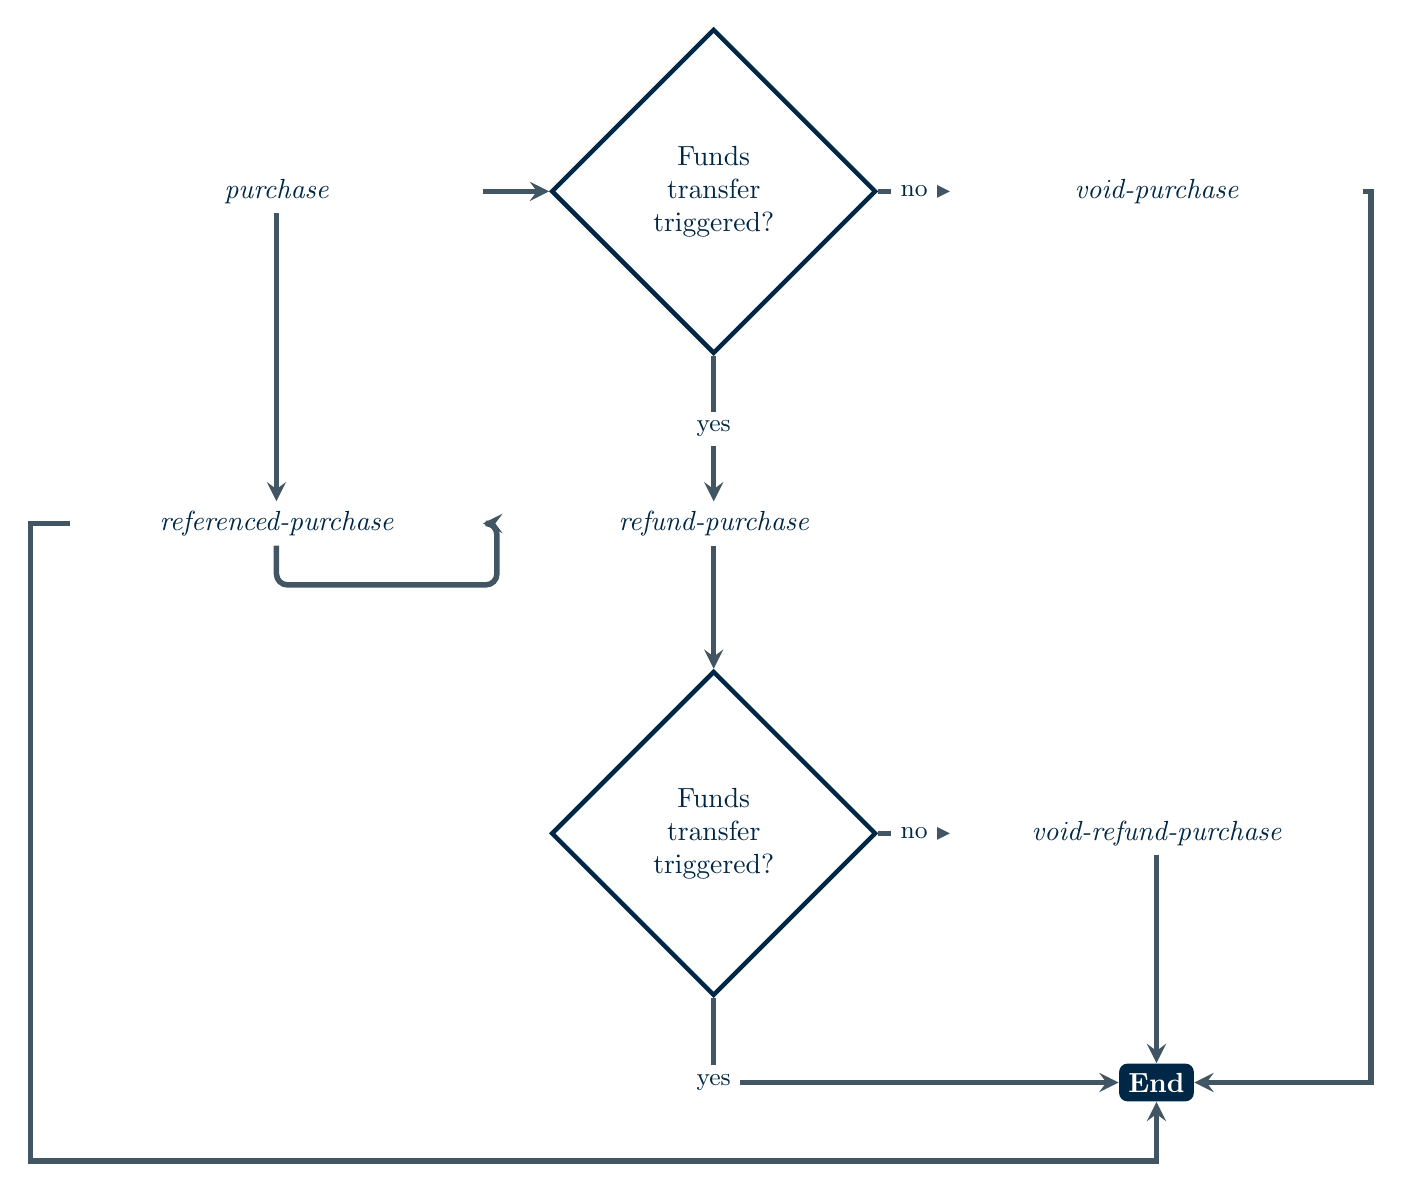
\begin{tikzpicture}

% Body
   % tx types
   \node [transaction] (purchase) at (0,0) {purchase};     
%   \node (Start) [start_end, above of= purchase, node distance=15] {Start};
   \node (decision1) [decision, right of= purchase, node distance=158] {Funds\\ transfer\\ triggered?};
   \node [transaction,right of= decision1, node distance=160] (void-purchase) {void-purchase};
   \node [transaction, below of= decision1, node distance=120] (refund-purchase) {refund-purchase};
   \node[transaction] (referenced-purchase) at (refund-purchase -| purchase) {referenced-purchase};
   \node (decision2) [decision, below of= refund-purchase, node distance=112] {Funds\\ transfer\\ triggered?};
      \node[transaction] (void-refund-purchase) at (decision2 -| void-purchase)  {void-refund-purchase};
   \node (end) [start_end, below of= void-refund-purchase, node distance=90] {End};
   
% Arrows & Text
  \draw [solidarrow, rounded corners] 
                           (referenced-purchase) |- ($(referenced-purchase.south) + (+2.8,-0.5)$) |- (referenced-purchase.east);
  \draw[solidarrow]
                           (referenced-purchase.west) -| ($(referenced-purchase.west) + (-0.5,-8.1)$) -| (end.south);
  \draw[solidarrow]
                      	(purchase.south) -| (referenced-purchase.north);
  \draw[solidarrow]
                      	(purchase.east) -- (decision1.west);
  \draw[solidarrow]
                      	(decision1.east) -- (void-purchase.west) node [yes_no] {no}; 
  \draw[solidarrow]
                      	(void-purchase.east) |- (13.9,-0) |-  (end.east);
  \draw[solidarrow]
                      	(decision1.south) -- (refund-purchase.north) node [yes_no] {yes};
  \draw[solidarrow]
                      	(refund-purchase.south) -- (decision2.north); 
  \draw[solidarrow]
                      	(decision2.east) -- (void-refund-purchase.west) node [yes_no] {no};
  \draw[solidarrow]
                      	(void-refund-purchase.south) -- (end.north);
  \draw[solidarrow]
                      	(decision2.south) |- (end.west) node [yes_no] {yes};                      	
                      
\end{tikzpicture}
\end{document}
